\documentclass[tikz]{standalone}
\usepackage{pgfplots}
\pgfplotsset{compat=1.15}
\usepackage{mathrsfs}
\usetikzlibrary{arrows,calc}
\usepackage{tkz-euclide}

\pagestyle{empty}

\definecolor{AngleClr}{rgb}{0,0.39215686274509803,0}
\definecolor{ShapeClr}{rgb}{0.6,0.2,0}
\definecolor{BlueClr}{RGB}{5,81,163}

\begin{document}

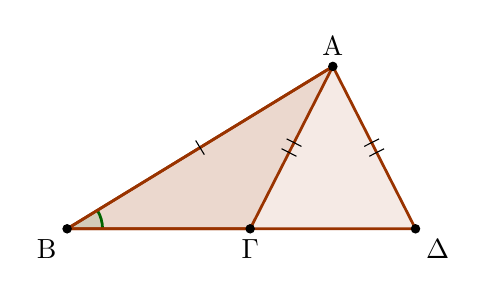
\begin{tikzpicture}[scale=.75]
\tkzSetUpLine[line width=1pt,color=black]
\tkzSetUpPoint[fill=black]

\tkzDefPoints{6/2.75/A,1.5/0/B,4.6/0/C,7.4/0/D}
% \tkzDefPoints{0/-4/E,1.1/-1.3/D,5/-3.6/Z}

\tkzFillPolygon[fill=ShapeClr,fill opacity=0.1](A,B,C)
\tkzFillPolygon[fill=ShapeClr,fill opacity=0.1](A,B,D)

\tkzFillAngle[fill=AngleClr,size=.6,fill opacity=0.1](C,B,A)
\tkzMarkAngle[line width=1pt,color=AngleClr,size=.6](C,B,A)
r,size=.4](A,C,B D,Z,E)


\tkzDrawPolygon[color=ShapeClr](A,B,C)
\tkzDrawPolygon[color=ShapeClr](A,B,D)

\tkzDrawPoints[size=3](A,B,C,D)

\tkzLabelPoint[above](A){$\rm A$}
\tkzLabelPoint[below left](B){$\rm B$}
\tkzLabelPoint[below](C){$\rm \Gamma$}
\tkzLabelPoint[below right](D){$\rm \Delta$}

\tkzMarkSegments[mark=|,size=3](A,B)
\tkzMarkSegments[mark=||,size=3](A,C A,D)

\end{tikzpicture}

\end{document}
